\section{question 2}

For the three values of $Q$ we now consider a situation with a finite excitation time such that $F(t) = F_0 cos(\omega t)$ for $t<0$ and $F(t) = 0$ for t =.

\begin{figure}[h!] 
	\centering
	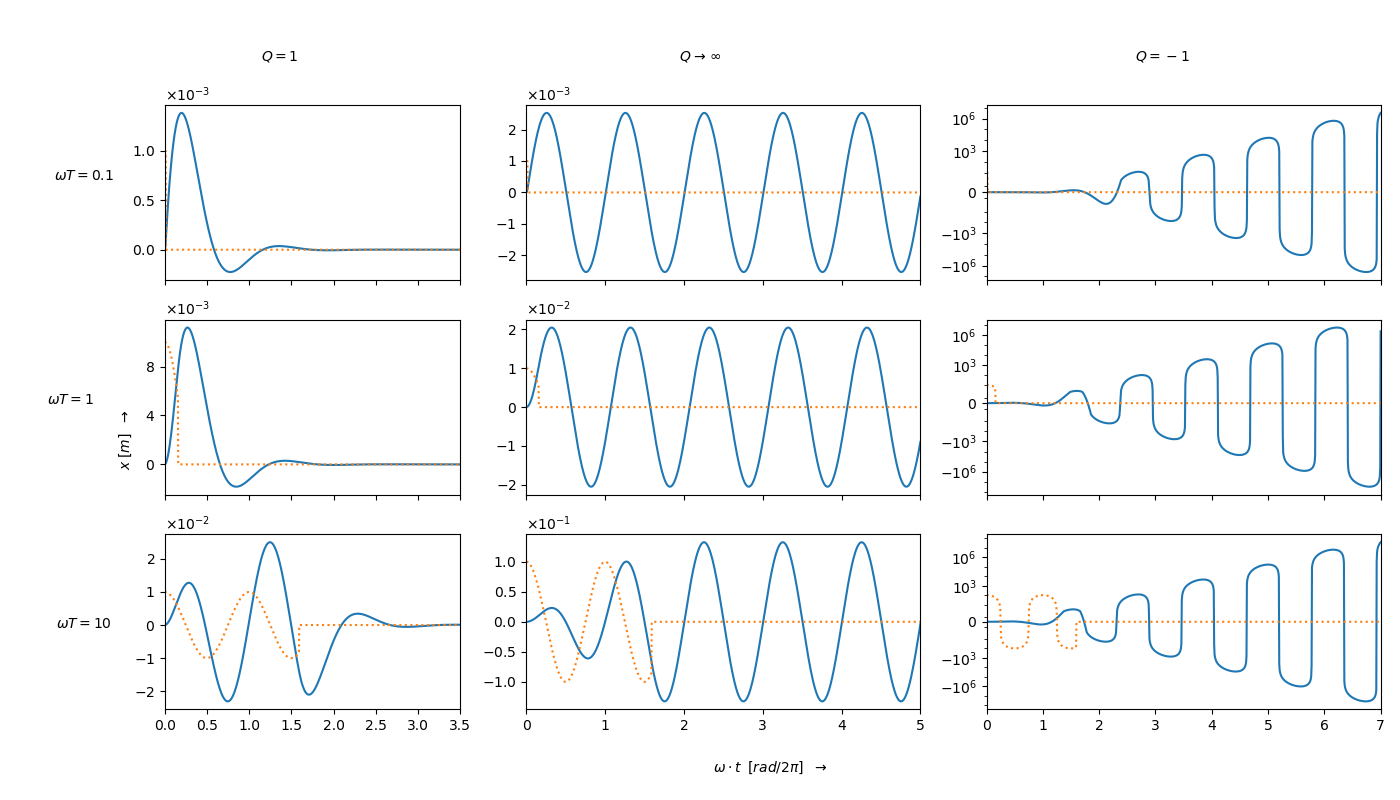
\includegraphics[width=0.6\textwidth]{figures/graph_q2.png}
	\caption{Graphs of $x(t)$ and $F(t)$  as function of $t$ for different values of $Q$. The solid blue lines correspond with $x(t)$ and the orange dashed lines correspond to a scaled version of $F(t)$.}
	\label{fig_q1}
\end{figure}